%\RequirePackage{etex}
\documentclass{book}

\usepackage[utf8]{inputenc}
\usepackage[russian]{babel}
\usepackage{epigraph}
\usepackage{fancyvrb}
\usepackage{amsfonts}
\usepackage{amsmath}
\usepackage{amssymb}
\usepackage{url}
\usepackage[dvips]{color}
\usepackage[arrow,curve,matrix,frame]{xy}
\usepackage{indentfirst}	% Русская типографика требует красную строку
%\usepackage{MnSymbol}
\usepackage{array}
\usepackage{ifmtarg}
\usepackage{centernot}
\usepackage{empheq}
\usepackage{needspace}
\usepackage{colonequals}
\usepackage{graphicx}
\usepackage{tikz}
\usetikzlibrary{arrows,positioning,shapes,shadows,trees}
%\usepackage{tikz-qtree}
\usepackage{mdwlist}
\usepackage{Khartiya}

%\usepackage{fancybox}
%% Я хотел использовать fancybox ради \ovalbox, но он определяет свой
%% собственный Verbatim, который конфликтует с fancyvrb.
%% В конце концов нужно будет либо выдернуть оттуда определение
%% \ovalbox, либо отказаться от fancyvrb. Пока что я просто не делаю
%% круглых углов.
\newcommand{\ovalbox}[1]{\fbox{#1}}

\setlength{\epigraphwidth}{7cm}

\usepackage{longtable,citehack,enumerate}
\usepackage{tocbibind}
%\usepackage[unicode,colorlinks=true,a4paper]{hyperref}
\usepackage[unicode,a4paper]{hyperref}
\definecolor{pfpcolorint}{rgb}{0,0.4,0}
\definecolor{pfpcolorext}{rgb}{0,0,0.6}

\hypersetup{colorlinks,
	linkcolor=pfpcolorint,
	citecolor=pfpcolorint,
	filecolor=pfpcolorext,
	urlcolor=pfpcolorext,
	bookmarksopen,bookmarksopenlevel=0,
	pdffitwindow,
	pdftitle={Магнус Лай Хетланд. Алгоритмы в Python},
	% pdfsubject={},
	% pdfkeywords={}
}

\interfootnotelinepenalty=10000
% 70х100/16 -> 170mmх240mm
\usepackage[papersize={165mm,240mm},hmargin={1.6cm,2cm},vmargin={2cm,2cm},twoside]{geometry}

\usepackage[dvipdfm]{accsupp} % Контролирует эффект копирования из PDF

% headers & footers
\usepackage{fancyhdr}
\pagestyle{fancy}
%\include{version}
\fancyhead{}
\fancyhead[LE,RO]{\slshape{\rightmark{}}}
%\fancyhead[LE,RO]{\thepage{}}
%\fancyfoot{}
%\fancyfoot[LE,RO]{rev. \svnInfoMaxRevision}
% 
\usepackage{graphicx}

\usepackage[round]{natbib}
\bibliographystyle{plainnat}
\renewcommand{\cite}{\citep*}
\newcommand{\citeterse}{\citep}
\newcommand{\citeyr}[1]{(\citeyear{#1})}
\newcommand{\citeyropen}[1]{\citeyear{#1}}
\newcommand{\fulllongcite}[1]{\citeauthor*{#1} \citeyearpar{#1}}
\newcommand{\citeopen}[1]{\citealp*{#1}}
\newcommand{\citeopenterse}[1]{\citealp{#1}}

%%\usepackage{algorithm}

\usepackage{listings}
\lstloadlanguages{Python,bash}
\definecolor{listingcomment}{gray}{0.3}
\lstset{%
  basicstyle=\small\ttfamily\upshape,
  showtabs=false, 
  showspaces=false, 
  showstringspaces=false,
  tabsize=2,
  language=Python,
  commentstyle=\color{listingcomment},
  extendedchars=\true{},
  mathescape=\true{},% allows to use math symbols in listings - may be
                     % dangerous
  keywordstyle={}}
% замена буквосочетаний на симпатичные символы
\lstset{literate={->}{{$\to{}$}}1 {=>}{{$\Rightarrow$}}2 {|>}{{$\triangleright{}$}}1}

% \lstinline мешается в таблицах (пока не понял, почему) -- goga
%\newcommand{\code}[1]{\lstinline[mathescape]!#1!}
\newcommand{\code}[1]{\texttt{#1}}

%% proper captions for figures, etc
\RequirePackage{caption}
\captionsetup{labelsep=period,labelfont=bf}

% Добавляем точку после номера раздела
\usepackage{titlesec}
\titlelabel{\thetitle.\quad}
\usepackage[dotinlabels]{titletoc}


% settings for floating objects
\renewcommand{\topfraction}{.9}
\renewcommand{\textfraction}{.1}
\renewcommand{\bottomfraction}{.9}
%\renewcommand{\floatpagefraction}{.9}
%\renewcommand{\dblfloatpagefraction}{\floatpagefraction}
% \setcounter{topnumber}{4}
% \setcounter{bottomnumber}{4}
% \setcounter{totalnumber}{4}
% \setlength{\floatsep}{8pt plus 2pt minus 2pt}
% \setlength{\textfloatsep}{8pt plus 2pt minus 2pt}
% \setlength{\intextsep}{12pt plus 2pt minus 2pt}

% Custom commands
\newcommand{\<}{\langle}
\renewcommand{\>}{\rangle}
\newcommand{\nbdash}{\mbox{-}}
\newcommand{\nosol}{\nrightarrow}
\newcommand{\recommended}{\textsc{Рекомендуется}}

\newcommand{\lambdaterm}[1]{\mbox{\code{#1}}}
\newcommand{\nbcode}[1]{\mbox{\code{#1}}}
\newcommand{\ocode}[1]{\overline{\vphantom{A}\code{#1}}}

\newcommand{\defterm}[1]{\emph{#1}}

\newcommand{\ruleid}[1]{\mbox{\textsc{#1}}}
\newcommand{\ruletag}[1]{\tag{\textsc{#1}}\index{правило!\textsc{#1}}}

\newcommand{\N}{\mathbb{N}}
\newcommand{\dom}{\textit{dom}}
\newcommand{\range}{\textit{range}}
\newcommand{\fail}{\textit{неудача}}
\newcommand{\function}[1]{\mbox{\textit{#1}\,}}
\newcommand{\interpreter}[1]{\texttt{#1}\index{интерпретатор!\texttt{#1}}}

\newcommand{\Fsub}{F$_{\code{<:}}$}
\newcommand{\Fomega}{F$_\omega$}
\newcommand{\Fsubomega}{F$_{\code{<:}}^\omega$}

\renewcommand{\L}{\ensuremath{\lambda}}

\newcommand{\eqdef}{\stackrel{\text{\tiny def}}{=}}

\newcommand{\size}[1]{\bar #1 \bar}

\newcommand{\varrow}{\mbox{\strut\ensuremath{\:\Mapstochar\shortrightarrow\:}}}
\newcommand{\notsub}{\ensuremath{\centernot{\code{\textnormal{<:}}}}}

\definecolor{gray}{gray}{0.75}
\newcommand{\graybg}[1]{\colorbox{gray}{\mbox{#1}}}

\makeatletter
\newcommand{\translationnotemark}{{\renewcommand{\@makefnmark}{\mbox{$^*$}}\footnotemark{}}}
\newcommand{\translationnotetext}[1]{{\renewcommand{\@makefnmark}{\mbox{$^*$}}\footnotetext{#1~---~{\it прим. перев.}}}\addtocounter{footnote}{-1}}
\newcommand{\translationnote}[1]{\translationnotemark{}\translationnotetext{#1}}
\newcommand{\unmarkednote}[1]{{\renewcommand{\@makefnmark}{}\footnotemark{}\footnotetext{#1}}\addtocounter{footnote}{-1}}
\makeatother

\newcommand{\wearelazy}{\translationnote{При верстке перевода это правило не соблюдалось.}}

\newtheorem{definition}{\texttt{Определение}}[section]
\newtheorem{exercise}[definition]{\texttt{Упражнение}}
\newtheorem{axiom}[definition]{\texttt{Аксиома}}
\newtheorem{proposition}[definition]{\texttt{Утверждение}}
\newtheorem{lemma}[definition]{\texttt{Лемма}}
\newtheorem{theorem}[definition]{\texttt{Теорема}}
\newtheorem{convention}[definition]{\texttt{Соглашение}}
\newtheorem{corollary}[definition]{\texttt{Следствие}}
\newtheorem{example}[definition]{\texttt{Пример}}
\newtheorem{examples}[definition]{\texttt{Примеры}}

\newcommand{\errata}[1]{\relax}

\newcommand{\muheight}{\ensuremath{\mu\mbox{-height}}}
\newcommand{\recordc}[4]{\ensuremath{\code{#1}_#2{}^{#2\in #3..#4}}}

\newenvironment{exsolution}[1]
  {\par\smallskip\noindent
   \ref{#1}. \textsc{Решение:}}{}

%%%
%%% НОВАЯ ВЕРСТКА ТАБЛИЦ
%%%
%%% сначала идёт параграф с заголовком...
\newcommand{\displayNew}[3]{#1

%%% ... потом верхняя рамка
\rule[-1ex]{.4pt}{1ex}\rule{\mapltablewidth}{.4pt}\rule[-1ex]{.4pt}{1ex}\smallskip

%%% ... потом две minipage, стоящие рядом через черточку
\begin{minipage}[t]{.5\mapltablewidth}
#2
\end{minipage}
\vline
\begin{minipage}[t]{.5\mapltablewidth}
#3
\end{minipage}

%%% ... потом нижняя рамка
\rule{.4pt}{1ex}\rule{\mapltablewidth}{.4pt}\rule{.4pt}{1ex}\par
}

\makeatletter
\newcommand{\tablesection}[2]{\textit{#1}\@ifmtarg{#2}{\relax}{\hfill\fbox{#2}}}
\makeatother

\newcommand{\displayOneCol}[2]{
  { % hold \arraystretch redefinition inside the display
    #1 \\
    \renewcommand{\arraystretch}{0}
    \begin{tabular}{|c|}
      \hline
      \rule{0pt}{1ex} \\
      \multicolumn{1}{c}{
        \renewcommand{\arraystretch}{1}
        \begin{tabular}{l}
          #2
        \end{tabular}
      } \\
      \rule{0pt}{1ex} \\
      \hline
    \end{tabular}
  }
}



\title{Алгоритмы в Python. Проектирование алгоритмов на языке Python}
\author{Магнус Лай Хетланд}

\begin{document}
\newlength{\mapltablewidth}
\setlength{\mapltablewidth}{\linewidth}
\addtolength\mapltablewidth{-2.8pt}
\VerbatimFootnotes
\selectlanguage{russian}%
\frenchspacing
\righthyphenmin=2
\sloppy
\setcounter{topnumber}{1}

\maketitle

%%% здесь можно комментировать одно и раскомментировать другое, чтобы
%%% быстро тестировать компиляцию по главам
%\input{chapter-13.tex}
\tableofcontents

\chapter*{Предисловие}
\addcontentsline{toc}{chapter}{Предисловие}

%This book is a marriage of three of my passions: algorithms, Python programming, and explaining
%things. To me, all three of these are about aesthetics—finding just the right way of doing something,
%looking until you uncover a hint of elegance, and then polishing that until it shines. Or at least until it is a
%bit shinier. Of course, when there’s a lot of material to cover, you may not get to polish things quite as
%much as you want. Luckily, though, most of the contents in this book is prepolished, because I’m writing
%about really beautiful algorithms and proofs, as well as one of the cutest programming languages out
%there. As for the third part, I’ve tried hard to find explanations that will make things seem as obvious as
%possible. Even so, I’m sure I have failed in many ways, and if you have suggestions for improving the
%book, I’d be happy to hear from you. Who knows, maybe some of your ideas could make it into a future
%edition? For now, though, I hope you have fun with what’s here and that you take any newfound insight
%and run with it. If you can, use it to make the world a more awesome place, in whatever way seems right.


Эта книга родилась как слияние трех моих увлечений: алгоритмов, программирования на Python и объяснения людям разных вещей. По мне эстетика подразумевает три действия: вы находите правильный способ сделать что-либо, приглядываетесь к нему до тех пор, пока не проявится намек на элегантность, а затем шлифуете его до блеска. Ну, или хотя бы делаете чуть красивее. Конечно, когда требуется выполнить очень много работы, вы, вероятно, не сможете довести свои решения до совершенства. К счастью, большая часть материалов в этой книге близка к совершенству, так как я описываю действительно прекрасные алгоритмы и доказательства и использую один из лучших языков программирования. Что же до третьей составляющей, я серьезно поработал, чтобы объяснить вещи так просто, как это только возможно. Но даже при этом, я уверен, что во многих местах этого не достиг, так что если у вас есть советы по улучшению книги, я буду рад их услышать. Кто знает, может быть какие-то из ваших идей могут войти в следующее издание? Сейчас же я надеюсь, что эта книга вам понравится и вдохновит вас двигаться дальше. Если вы можете, используйте ее, чтобы сделать мир чуточку лучше.
%%% Local Variables: 
%%% mode: latex
%%% TeX-master: "mapl"
%%% End: 


\chapter{Введение}
\label{chap:intro}

\epigraph{
1. Запишите задачу на бумаге.\\
2. Подумайте действительно хорошенько.\\
3. Запишите решение задачи.
}{<<Алгоритм Фейнмана>>, по Мюррею Гелл-Манну.}


Представьте себе такую задачу. Вам нужно посетить все города, городки и поселки, например, Швеции и вернуться в исходную точку. Это может занять немало времени (ведь нужно заглянуть в 27 978 мест), так что Вам хочется сделать маршрут покороче. Вы собираетесь заехать в каждое место только один раз следуя кратчайшим путем. Будучи программистом Вы точно не собираетесь рисовать маршрут вручную. Вместо этого Вы попробуете написать программу, которая все рассчитает сама. Однако, по какой-то причине Вам это никак не удается. Очевидное решение неплохо работает на небольшом количестве городов, но на реальной задаче расчет никак не завершается, а улучшить программу оказывается неожиданно сложно. Как быть?

Между тем, в 2004-ом году команда из 5 исследователей\footnote{David Applegate, Robert Bixby, Vašek Chvátal, William Cook, and Keld Helsgaun} нашла такой путь по Швеции, после того как несколько подобных проектов завершились неудачей. Эта команда использовала самое новое ПО с кучей хитрых оптимизаций, запущенное на кластере из 96 машин на Xeon 2.6ГГц. Их программа проработала с марта 2003-го до мая 2004-го, прежде чем было получено оптимальное решение. Ребята посчитали, что с учетом разных перерывов общее процессорное время, потраченное на решение задачи, оказалось равным \textit{85 годам}!

Представьте теперь похожую задачу: из Кашгара, на самого западе Китая, Вам нужно попасть в Нинбо, на восточное побережье, следуя кратчайшем путем. В Китае 3 583 715 км автомобильных и 77 384 км железных дорог, которые пересекаются в миллионах мест и образуют неисчислимое количество возможных маршрутов. Может показаться, что эта проблема аналогична предыдущей, но уже сейчас такая задача \textit{поиска кратчайшего пути} решается без каких-либо затруднений и задержек GPS-навигаторами и онлайн-картами. Если Вы отметите два этих города на любимом картографическом сервисе, то получите кратчайший маршрут за пару мгновений. Так в чем же тут дело?

Дальше в книге Вы узнаете больше о двух этих задачах. Первая называется \textit {проблемой коммивояжера} и описана в главе \ref{chap:hard-problems}, а так называемая проблема поиска кратчайшего пути рассматривается в главе \ref{chap:from-a-to-b}. Я надеюсь, что Вы начнете хорошо понимать, почему одни задачи так сложны для решения, в то время как другие имеют несколько известных и эффективных решений. Что еще важнее, Вы научитесь работать с любыми вычислительными и алгоритмическими задачами, либо эффективно решая их, используя описанные в книге техники и алгоритмы, либо показывая, что они слишком сложны, и приближенное решение "--- это лучшее, на что можно рассчитывать. Эта глава вкратце описывает всю книгу: что Вы можете от нее получить и что требуется от Вас. В ней также обозначены темы остальных глав, чтобы Вы могли читать их выборочно.


\begin{lstlisting}[caption={An Iterative Solution to the Longest Common Subsequence (LCS)}]
def lcs(a,b):
    n, m = len(a), len(b)
    pre, cur = [0]*(n+1), [0]*(n+1) # Previous/current row
    for j in range(1,m+1): # Iterate over b
        pre, cur = cur, pre # Keep prev., overwrite cur.
        for i in range(1,n+1): # Iterate over a
            if a[i-1] == b[j-1]: # Last elts. of pref. equal?
                cur[i] = pre[i-1] + 1 # L(i,j) = L(i-1,j-1) + 1
            else: # Otherwise...
                cur[i] = max(pre[i], cur[i-1]) # max(L(i,j-1),L(i-1,j))
    return cur[n] # L(n,m)
\end{lstlisting}


%%% Local Variables: 
%%% mode: latex
%%% TeX-master: "mapl"
%%% End: 
 %% Introduction
\chapter{Основы}
\label{chap:basics}

\epigraph{Трейси: Я не знал, что ты была там.\\
Зоуи: В каком-то смысле. Невидимость — ты, вероятно, слышал о ней.\\
Трейси: Не думаю, что это было в базовом курсе.
}{Из 14-го эпизода <<Firefly>>, <<Сообщение>>}



\section{Некоторые базовые понятия в вычислениях}

\section{Асимптотическая нотация}
\subsection{Это какая-то китайская грамота!}
\subsection{Основные термины и правила}
\subsection{Take the Asymptotics for a Spin }
\subsection{Three Important Cases}
\subsection{Эмпирическая оценка алгоритмов}
\label{sec:empirical-evaluation}

В этой книге описывается\textit{ проектирование алгоритмов} (и тесно связанный с ним\textit{ анализ алгоритмов}). Но в разработке есть также и другой немаловажный процесс, жизненно необходимый при создании крупных реальных проектов, это — \textit{оптимизация алгоритмов}, искусство их \textit{эффективной реализации}. С точки зрения такого разделения, проектирование алгоритма можно рассматривать как способ достижения низкой асимптотической сложности алгоритма (с помощью разработки эффективного алгоритма), а оптимизацию — как уменьшение констант, скрытых в этой асимптотике.

Хотя я могу дать несколько советов по алгоритмам проектирования в Python, сложно угадать, какие именно хитрости и уловки дадут вам лучшую производительность в конкретной задаче, над которой вы работаете, или для вашего оборудования и версии Python. (Асимптотики используются как раз для того, чтобы не было нужды прибегать к таким вещам). Вообще, в некоторых случаях хитрости могут вовсе не потребоваться, потому что ваша программа и так достаточно быстра. Самое простое, что вы можете сделать в большинстве случаев, это просто пробовать и смотреть. Если у вас \textit{есть идея} какого-то хака, то просто опробуйте ее! Реализуйте свою хитрость и запустите несколько тестов. Есть ли улучшения? А если это изменение делает ваш код менее читаемым, а прирост производительности мал, то подумайте — стоит ли оно того?

\begin{note}
Этот раздел рассказывает об оценке алгоритмов, а не об их оптимизации. В приложении \ref{app:A} есть несколько советов по ускорению программ на Python.
\end{note}

Есть ряд теоретических аспектов так называемой экспериментальной алгоритмики (то есть, экспериментальной оценки алгоритмов и их реализации), но они выходят за рамки этой книги, так что я дам вам несколько практических советов, которые могут быть весьма полезны.

\subsubsection*{Совет 1. Если возможно, то не беспокойтесь об этом}

Беспокойство об асимптотической сложности может быть очень полезным. Иногда \textit{решение} задачи из-за сложности на практике может \textit{перестать} быть таковым. Однако, постоянные константы в асимптотике часто совсем не критичны. Попробуйте простую реализацию алгоритма для начала, и убедитесь, что она работает стабильно. (В принципе, вы можете сначала попробовать примитивный алгоритм. Гуру программирования Кен Томпсон писал: «Когда вы в затруднении, используйте перебор вариантов». Перебор вариантов в алгоритмах обычно означает попытку попробовать каждое из возможных решений, при этом временные затраты будут безумными!) Если все работает — оставьте как есть.

\subsubsection*{Совет 2. Для измерения времени работы используйте \texttt{timeit}}

Модуль \texttt{timeit} предназначен для измерения времени работы. Хотя для получения действительно надежных данных вам потребуется выполнить кучу работы, для практических целей timeit вполне сгодится. Например:

\begin{lstlisting}
>>> import timeit
>>> timeit.timeit("x = 2 + 2")
0.034976959228515625
>>> timeit.timeit("x = sum(range(10))")
0.92387008666992188
\end{lstlisting}

Модуль timeit можно использовать прямо из командной строки, например:

\begin{lstlisting}
python -m timeit -s"import mymodule as m" "m.myfunction()"
\end{lstlisting}

Существует кое-что, с чем вы должны быть осторожны при использовании \texttt{timeit}: побочные эффекты, которые будут влиять на повторное исполнение \texttt{timeit}. Функция \texttt{timeit} будет запускать ваш код несколько раз, чтобы увеличить точность, и если прошлые запуски влияют на последующие, то вы окажетесь в затруднительном положении. Например, если вы измеряете скорость выполнения чего-то вроде \texttt{mylist.sort()}, список будет отсортирован только \textit{в первый раз}. Во время остальных тысяч запусков список уже будет отсортированным и это даст нереально маленький результат.

Больше информации об этом модуле и о том, как он работает, можно найти в документации стандартной библиотеки Python.

\subsubsection*{Совет 3. Чтобы найти узкие места, используйте профайлер}

Часто, для того чтобы понять, какие части программы требуют оптимизации, делаются разные догадки и предположения. Такие предположения нередко оказываются ошибочными. Вместо того, чтобы гадать, воспользуйтесь профайлером. В стандартной поставке Python идет несколько профайлеров, но рекомендуется использовать \texttt{cProfile}. Им так же легко пользоваться, как \texttt{timeit}, но он дает больше подробной информации о том, на что тратится время при выполнении программы. Если основная функция вашей программы называется \texttt{main}, вы можете использовать профайлер следующим образом:

\begin{lstlisting}
import cProfile
cProfile.run('main()')
\end{lstlisting}

Такой код выведет отчет о времени работы различных функций программы. Если в вашей системе нет модуля \texttt{cProfile}, используйте \texttt{profile} вместо него. Больше информации об этих модулях можно найти в документации. Если же вам не так интересны детали \textit{реализации}, а просто нужно оценить поведение \textit{алгоритма} на конкретном наборе данных, воспользуйтесь модулем \texttt{trace} из стандартной библиотеки. С его помощью можно посчитать, сколько раз будут выполнены то или иное выражение или вызов в программе.

\subsubsection*{Совет 4. Показывайте результаты графически}

Визуализация может стать прекрасным способом, чтобы понять что к чему. Для исследования производительности часто применяются \textit{графики} (например, для оценки связи количества данных и времени исполнения) и диаграммы типа \textit{<<ящик с усами>>}, отображающие распределение временных затрат при нескольких запусках. Примеры можно увидеть на рисунке \ref{fig:evaluation-diagrams}.

\begin{figure}[h]
	\centering
	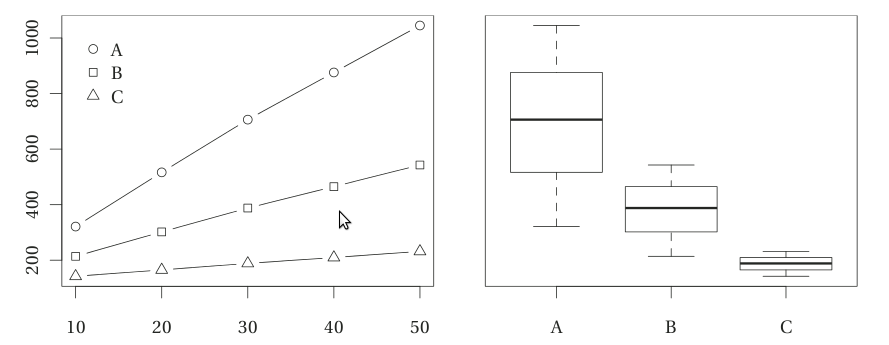
\includegraphics[width=\textwidth]{img/2-2.png}
	\caption{Визуализация времени работы для программ A, B и C и размеров данных 10 "--- 50}
	\label{fig:evaluation-diagrams}
\end{figure}

Отличная библиотека для построения графиков и диаграмм из Python "--- matplotlib (можно взять на http://matplotlib.sf.net).

\subsubsection*{Совет 5. Будьте внимательны в выводах, основанных на сравнении времени работы}

Этот совет довольно расплывчатый, потому что существует много ловушек, в которые можно попасть, делая выводы о том, какой способ лучше, на основании сравнения времени работы. Во-первых, любая разница, которую вы видите, может определяться случайностью. Если вы используете специальные инструменты вроде \texttt{timeit}, риск такой ситуации меньше, потому что они повторяют измерение времени вычисления выражения несколько раз (или даже повторяют весь замер несколько раз, выбирая лучший результат). Таким образом, всегда будут случайные погрешности и если разница между двумя реализациями не превышает некоторой погрешности, нельзя сказать, что эти реализации различаются (хотя и то, что они одинаковы, тоже \textit{нельзя} утверждать).

\begin{note}
Если вам нужно сделать выводы быстро, можно воспользоваться методом проверки статистических гипотез. Однако, на практике, если различия действительно очень малы, то, вероятно, неважно, какую реализацию вы выберете, так что используйте ту, что больше нравится.
\end{note}

Проблема усложняется, если вы сравниваете больше двух реализаций. Количество пар для сравнения увеличивается пропорционально \textit{квадрату} количества сравниваемых версий, \textit{сильно} увеличивая вероятность того, что как минимум две из версий будут казаться слегка различными. (Это называется проблемой \textit{множественного сравнения}). Существуют статистические решения этой проблемы, но самый простой способ "--- повторить эксперимент с двумя подозрительными версиями. Возможно, потребуется сделать это несколько раз. Они по-прежнему выглядят похожими?

Во-вторых, есть несколько моментов, на которые нужно обращать внимание при сравнении средних величин. Как минимум, вы должны сравнивать средние значения реального времени работы. Обычно, чтобы получить показательные числа при измерении производительности, время работы каждой программы нормируется делением на время выполнения какого-нибудь стандартного, простого алгоритма. Действительно, это может быть полезным, но в ряде случаев сделает бессмысленными результаты замеров. Несколько полезных указаний на эту тему можно найти в статье <<How not to lie with statistics: The correct way to summarize benchmark results>> Fleming и Wallace. Также можно почитать Bast и Weber <<Don't compare averages>>, или более новую статью Citron и др. <<The harmonic or geometric mean: does it really matter?>>

И в-третьих, возможно, ваши выводы нельзя обобщать. Подобные измерения на другом наборе входных данных и на другом железе могут дать другие результаты. Если кто-то будет пользоваться результатами ваших измерений, \textit{необходимо последовательно задокументировать}, каким образом вы их получили.

\subsubsection*{Совет 6. Будьте осторожны, делая выводы об асимптотике из экспериментов}

Если вы хотите что-то сказать окончательно об асимптотике алгоритма, то необходимо проанализировать ее, как описано ранее в этой главе. Эксперименты могут дать вам намеки, но они очевидно проводятся на конечных наборах данных, а асимптотика "--- это то, что происходит при сколь угодно больших размерах данных. С другой стороны, если только вы не работаете в академической сфере, \textit{цель} асимптотического анализа "--- сделать какой-то вывод о поведении алгоритма, реализованного конкретным способом и запущенного на определенном наборе данных, а это значит, что измерения \textit{должны быть} соответствующими.

Например, вы \textit{предполагаете}, что алгоритм работает с квадратичной сложностью, но вы не можете окончательно доказать это. Можете ли вы использовать эксперименты для доказательства вашего предположения? Как уже говорилось, эксперименты (и оптимизация алгоритмов) имеют дело в основном с постоянными коэффициентами, но \textit{выход есть}. Основной проблемой является то, что ваша гипотеза на самом деле непроверяема экспериментально. Если вы утверждаете, что алгоритм имеет сложность $O(n^2)$, то данные не могут это ни подтвердить, ни опровергнуть. Тем не менее, если вы сделаете вашу гипотезу более \textit{конкретной}, то она станет проверяемой. Вы могли бы, например, основываясь на некоторых данных положить, что время работы программы никогда не будет превышать $0.24n^2+0.1n+0.03$ секунд в вашем окружении. Это проверяемая (точнее, \textit{опровергаемая}) гипотеза. Если вы сделали множество измерений, но так и не можете найти контр-примеры, значит ваша гипотеза может быть верна. А это уже и подтверждает гипотезу о квадратичной сложности алгоритма.

\section{Реализация графов и деревьев }
\label{sec:implementing-graphs-and-trees}
Первая задача из главы \ref{chap:intro}, в которой нам требовалось объехать Швецию и Китай, была примером задачи, которая может быть решена с помощью одного из мощнейших инструментов "--- с помощью \textit{графов}. Часто, если вы можете определить, что решаете задачу на графы, вы по-крайней мере на полпути к решению. А если ваши данные можно каким-либо образом представить как \textit{деревья}, у вас есть все шансы построить действительно \textit{эффективное} решение.

Графами можно представить любую структуру или систему, от транспортной сети до сети передачи данных и от взаимодействия белков в ядре клетке до связей между людьми в Интернете.
Ваши графы могут стать еще полезнее, если вы добавите в них дополнительные данные вроде \textit{весов} или \textit{расстояний}, что даст возможность описывать такие разнообразные проблемы как игру в шахматы или определение подходящей работы для человека в соответствии с его способностями.
Деревья — это просто особый вид графов, так что большинство алгоритмов и представлений графов сработают и для них.
Однако, из-за их особых свойств (связанность и отсутствие циклов), можно применить специальные (и весьма простые) версии алгоритмов и представлений.
На практике в некоторых случаях встречаются структуры (такие как XML-документы или иерархия каталогов), которые могут быть представлены в виде деревьев\footnote{С учетом атрибутов IDREF и символьных ссылок XML-документы и иерархия каталогов становятся собственно графами.}. На самом деле эти <<некоторые>> случаи довольно-таки общие.

Если вы забыли терминологию (или ее и не знали), почитайте приложение \ref{app:graph-theory}, <<Терминология теории графов>>. Здесь же опишем основные моменты:

\begin{itemize}
\item Граф $G = (V, E)$ состоит из \textit{вершин}, $V$, и \textit{ребер} между ними, $E$. Если ребра имеют направление, то граф называется \textit{направленным}.
\item Вершины, связанные ребром, называются \textit{смежными}. Соединяющее две вершины ребро называется \textit{инцидентным} с ними. Вершины, смежные с $v$ называются \textit{соседними} с $v$.
\item \textit{Подграф} графа $G = (V,E)$ состоит из подмножества $V$ и подмножества $E$. \textit{Путь} в графе "--- это подграф, вершины которого соединены ребрами последовательно, причем каждая вершина включена только один раз. \textit{Цикл} — это то же самое, что и путь, только последнее его ребро связывает последнюю вершину с первой.
\item Если каждому ребру в $G$ будет сопоставлено определенное значение (\textit{вес}), то $G$ будет называться \textit{взвешенным} графом. \textit{Длина} пути или цикла — это сумма всех весов его ребер или, для невзвешенных графов, просто количество ребер.
\item \textit{Лесом} называется граф без циклов, а связанный граф — это \textit{дерево}. Иными словами, лес состоит из одного или многих деревьев.
\end{itemize}

Описание задачи в терминах графов является довольно абстрактным, так что если вам нужно реализовать решение, вы должны представить графы в виде каких-либо структур данных.

\subsection{Adjacency Lists and the Like}
\subsection{Матрицы смежности}
\label{sec:adjacency-matrix}

Другая распространенная форма представления графов — это матрицы смежности. Основное отличие их в следующем: вместо перечисления всех смежных с каждой из вершин, мы записываем один ряд значений (массив), каждое из которых соответствует возможной смежной вершине (есть хотя бы одна такая для каждой вершины графа), и сохраняем значение (в виде \texttt{True} или \texttt{False}), показывающее, действительно ли вершина является смежной. И вновь простейшую реализацию можно получить используя вложенные списки, как видно из листинга \ref{lst:adjacency}. Заметьте, что это также требует, чтобы вершины были пронумерованы от $0$ до $V-1$. В качестве значений истинности используются 1 и 0 (вместо \texttt{True} и \texttt{False}), чтобы сделать матрицу читабельной.

\begin{lstlisting}[caption={Матрица смежности, реализованная с помощью вложенных списков},label={lst:adjacency}]
a, b, c, d, e, f, g, h = range(8)
	    # a b c d e f g h

N = [[0,1,1,1,1,1,0,0], # a
		 [0,0,1,0,1,0,0,0], # b
		 [0,0,0,1,0,0,0,0], # c
		 [0,0,0,0,1,0,0,0], # d
		 [0,0,0,0,0,1,0,0], # e
		 [0,0,1,0,0,0,1,1], # f
		 [0,0,0,0,0,1,0,1], # g
		 [0,0,0,0,0,1,1,0]] # h
\end{lstlisting}

Способ использования матриц смежности слегка отличается от списков и множеств смежности. Вместо проверки, входит ли $b$ в $N[a]$, вы будете проверять, истинно ли значение ячейки матрицы $N[a][b]$. Кроме того, больше нельзя использовать $len(N[a])$, чтобы получить количество смежных вершин, потому что все ряды одной и той же длины. Вместо этого можно использовать функцию \texttt{sum}:
\begin{lstlisting}
>>> N[a][b]
1
>>> sum(N[f])
3
\end{lstlisting}

Матрицы смежности имеют ряд полезных свойств, о которых стоит знать. Во-первых, так как мы не рассматриваем графы с петлями (т.е. не работаем с псевдографами), все значения на диагонали — ложны. Также, ненаправленные графы обычно описываются парами ребер в обоих направлениях. Это значит, что матрица смежности для ненаправленного графа будет симметричной.

Расширение матрицы смежности для использования весов тривиально: вместо сохранения логических значений, сохраняйте значения весов. В случае с ребром $(u, v)$ $N[u][v]$ будет весом ребра $w(u,v)$ вместо \texttt{True}. Часто в практических целях несуществующим ребрам присваиваются бесконечные веса. (Это гарантирует, что они не будут включены, например, в кратчайшие пути, т. к. мы ищем путь по существующим ребрам). Не всегда очевидно, как представить бесконечность, но совершенно точно есть несколько разных вариантов.

Один из них состоит в том, чтобы использовать некорректное для веса значение, такое как \texttt{None} или $-1$, если известно, что все веса неотрицательны. Возможно, в ряде случаев полезно использовать действительно большие числа. Для целых весов можно применить \texttt{sys.maxint}, хотя это значение и не обязательно самое большое (длинные целые могут быть больше). Есть и значение, введенное для отражения бесконечности: \texttt{inf}. Оно недоступно в Python напрямую по имени и выражается как \texttt{float('inf')}\footnote{Гарантируется, что это работает для Python 2.6 и старше. В ранних версиях подобные специальные значения были платформо-зависимы, хотя \texttt{float('inf')} или \texttt{float('Inf')} должны сработать на большинстве платформ.}.

Листинг \ref{lst:adjacency-weighted} показывает, как выглядит матрица весов, реализованная вложенными списками. Использованы те же веса, что и в листинге \ref{lst:adjlist-weighted}.

\begin{lstlisting}[caption={Матрица весов с бесконечными значениями для отсутствующих ребер}, label={lst:adjacency-weighted}]
a, b, c, d, e, f, g, h = range(8)
_ = float('inf')

		# a b c d e f g h

W = [[0,2,1,3,9,4,_,_], # a
	 	 [_,0,4,_,3,_,_,_], # b
		 [_,_,0,8,_,_,_,_], # c
		 [_,_,_,0,7,_,_,_], # d
		 [_,_,_,_,0,5,_,_], # e
		 [_,_,2,_,_,0,2,2], # f
		 [_,_,_,_,_,1,0,6], # g
		 [_,_,_,_,_,9,8,0]] # h
\end{lstlisting}

Бесконечное значение обозначено как подчеркивание (\texttt{\_}), потому что это коротко и визуально различимо. Естественно, можно использовать любое имя, которое вы предпочтете. Обратите внимание, что значения на диагонали по-прежнему равны нулю, потому что даже без учета петель, веса часто интерпретируются как расстояния, а расстояние от вершины до самой себя равно нулю.

Конечно, матрицы весов дают возможность очень просто получить веса ребер, но, к примеру, проверка смежности и определение степени вершины, или обход всех смежных вершин делаются иначе. Здесь нужно использовать бесконечное значение, примерно так (для большей наглядности определим \texttt{inf = float('inf')}):
\begin{lstlisting}
>>> W[a][b] < inf
True
# смежность
>>> W[c][e] < inf
False
# смежность
>>> sum(1 for w in W[a] if w < inf) - 1 # степень
5
\end{lstlisting}

Заметьте, что из полученной степени вычитается $1$, потому что мы не считаем значения на диагонали. Сложность вычисления степени тут $\Theta(n)$, в то время как в другом представлении и принадлежность, и степень вершины можно определить за константное время. Так что  вы всегда должны понимать, \textit{как именно} вы собираетесь использовать ваш граф и выбирать для него соответствующее представление.

%%% BLACKBOX
\textbf{Массивы специального назначения из NumPy}

Библиотека NumPy содержит много функциональности, связанной с многомерными массивами. Для представления графов большая ее часть не нужна, но массивы из NumPy весьма полезны, например, для реализации матриц весов или смежности.

Вместо создания пустой матрицы весов или смежности из списков для $n$ вершин, вроде такого:
\begin{lstlisting}
>>> N = [[0]*10 for i in range(10)]
\end{lstlisting}
в NumPy можно использовать функцию \texttt{zeros}:
\begin{lstlisting}
>>> import numpy as np
>>> N = np.zeros([10,10])
\end{lstlisting}

Отдельные элементы доступны по индексам, разделенным запятой: $A[u,v]$. Чтобы получить соседние с данной вершины, используется одиночный индекс: $A[u]$.

Пакет NumPy можно получить по адресу http://numpy.scipy.org.

Имейте ввиду, что вам нужна та версия NumPy, что будет работать с вашей версией Python. Если последний релиз NumPy не поддерживает ту версию Python, что вы используете, вы можете скомпилировать и установить библиотеку прямо из репозитория исходных кодов. Исходный код можно получить с помощью следующих команд (предполагается, что у вас установлена Subversion):

\texttt{svn co http://svn.scipy.org/svn/numpy/trunk numpy}

Больше информации о том, как компилировать и устанавливать NumPy, так же как и подробную документацию, можно найти на сайте библиотеки.

\subsection{Реализация деревьев}

Любое представление графов, естественно, можно использовать для представления деревьев, потому что деревья "--- это особый вид графов. Однако, деревья играют свою большую роль в алгоритмах, и для них разработано много соответствующих структур и методов. Большинство алгоритмов на деревьях (например, поиск по деревьям, описанный в главе \ref{chap:divide-combine}) можно рассматривать в терминах теории графов, но специальные структуры данных делают их проще в реализации. 

Проще всего описать представление дерева с корнем, в котором ребра спускаются вниз от корня. Такие деревья часто отображают иерархическое ветвление данных, где корень отображает все объекты (которые, возможно, хранятся в листьях), а каждый внутренний узел показывает объекты, содержащиеся в дереве, корень которого "--- этот узел. Это описание можно использовать, представив каждое поддерево списком, содержащим все его поддеревья-потомки. Рассмотрим простое дерево, показанное на рисунке \ref{fig:simple-tree}.

Мы можем представить это дерево как список списков:
\begin{lstlisting}
>>> T = [["a", "b"], ["c"], ["d", ["e", "f"]]]
>>> T[0][1]
'b'
>>> T[2][1][0]
'e'
\end{lstlisting}

Каждый список в сущности является списком потомков каждого из внутренних узлов. Во втором примере мы обращаемся к третьему потомку корня, затем ко второму его потомку и в конце концов "--- к первому потомку предыдущего узла (этот путь отмечен на рисунке).


\tikzstyle{tree} = [circle,
						fill=white!90!black!10,
						drop shadow]
\begin{figure}[h]
\centering
\begin{tikzpicture}[level/.style={sibling distance=30mm/#1}]
    \tikzstyle{every node}=[circle,draw]
    \node[tree,draw=red] (z) {}
        child { 
			node[tree] {}
			child { node[tree] {\Large $a$} }
			child {	node[tree] {\Large $b$} } 
		}
        child {
            node[tree] {}
			child { node[tree] {\Large $c$} }
        }
        child { 
			node[tree,draw=red] (1) {} 
			child { node[tree] {\Large $d$} }
			child { 
				node[tree,draw=red] (2) {}
				child { node[tree,draw=red] (3) {\Large $e$} }
				child { node[tree] {\Large $f$} }
			}
		}
    ;
	\draw[-latex,color=red] (z) .. controls +(east:0.5cm) and +(north:1.5cm) .. (1) {};
	\draw[-latex,color=red] (1) .. controls +(right:0.3cm) and +(north:1cm) .. (2) {};
	\draw[-latex,color=red] (2) .. controls +(left:0.3cm) and +(north:1cm) .. (3) {};
\end{tikzpicture}
\caption{Пример дерева с отмеченным путем от корня к листу}
\label{fig:simple-tree}
\end{figure}


В ряде случаев возможно заранее определить максимальное число потомков каждого узла. (Например, каждый узел \textit{бинарного дерева} может иметь до двух потомков). Поэтому можно использовать другие представления, скажем, объекты с отдельным атрибутом для каждого из потомков как в листинге \ref{lst:binary-tree}.

\begin{figure}[h!]
\begin{lstlisting}[caption={Класс бинарного дерева}, label={lst:binary-tree}]
class Tree:
	def __init__(self, left, right):
	self.left = left
	self.right = right

You can use the Tree class like this:

>>> t = Tree(Tree("a", "b"), Tree("c", "d"))
>>> t.right.left
'c'
\end{lstlisting}
\end{figure}

Для обозначения отсутствующих потомков можно использовать \texttt{None} (в случае если у узла только один потомок). Само собой, можно комбинировать разные методы (например, использовать списки или множества потомков для каждого узла).

\newpage
\subsection{Множество разных представлений}

\section{Beware of Black Boxes}
\subsection{Hidden Squares}
\subsection{The Trouble with Floats}
\section{Заключение}
\section{Если вы заинтересовались…}
\section{Упражнения}
\section{Ссылки}





%%% Local Variables: 
%%% mode: latex
%%% TeX-master: "mapl"
%%% End: 
 %% The Basics
\chapter{Tangled Dependencies and Memoization}
\label{chap:memoization}
\epigraph{Twice, adv. Once too often.}{"--- Ambrose Bierce, The Devil's Dictionary}

Many of you may know the year 1957 as the birth year of programming languages\footnote{This was the year the first FORTRAN compiler was released by John Backus's group. Many consider this the first complete compiler, although the first compiler ever was written in 1942, by Grace Hopper.
}. For algorists, a possibly even more significant event took place this year: Richard Bellman published his groundbreaking book \textit{Dynamic Programming}. Although Bellman's book is mostly mathematical in nature, not really aimed at programmers at all (perhaps understandable, given the timing), the core ideas behind his techniques have laid the foundation for a host of very powerful algorithms, and they form a solid design method that any algorithm designer needs to master.

The term \textit{dynamic programming} (or simply DP) can be a bit confusing to newcomers. Both of the words are used in a different way than most might expect. \textit{Programming} here refers to making a set of choices (as in "linear programming") and thus has more in common with the way the term is used in, say, television, than in writing computer programs. \textit{Dynamic} simply means that things change over time"---in this case, that each choice depends on the previous one. In other words, this "dynamicism" has little to do with the program you'll write and is just a description of the problem class. In Bellman's own words, "I thought dynamic programming was a good name. It was something not even a Congressman could object to. So I used it as an umbrella for my activities."\footnote{See Richard Bellman on the Birth of Dynamic Programming in the references.}

The core technique of DP, when applied to algorithm design, is caching. You decompose your problem recursively/inductively just like before"---but you allow overlap between the subproblems. This means that a plain recursive solution could easily reach each base case an exponential number of times; however, by caching these results, this exponential waste can be trimmed away, and the result is usually both an impressively efficient algorithm \textit{and} a greater insight into the problem.

Commonly, DP algorithms turn the recursive formulation upside down, making it iterative, and filling out some data structure (such as a multidimensional array) step by step. Another option"---one I think is particularly suited to high-level languages such as Python"---is to implement the recursive formulation directly but to cache the return values. If a call is made more than once with the same arguments, the result is simply returned directly from the cache. This is called \textit{memoization}.

\begin{note}
Although I think memoization makes the underlying principles of DP clear, I do consistently rewrite the memoized versions to iterative programs throughout the chapter. While memoization is a great first step, one that gives you increased insight as well as a prototype solution, there are factors (such as limited stack depth and function call overhead) that may make an iterative solution preferable in some cases.
\end{note}

The basic ideas of DP are quite simple, but they can take a bit getting used to. According to Eric V. Denardo, another authority on the subject, "most beginners find all of them strange and alien." I'll be trying my best to stick to the core ideas and not get lost in formalism. Also, by placing the main emphasis on recursive decomposition and memoization, rather than iterative DP, I hope the link to all the work we've done so far in the book should be pretty clear.

Before diving into the chapter, here's a little puzzle: say you have a sequence of numbers, and you want to find its \textit{longest increasing} (or, rather \textit{nondecreasing} ) subsequence"---or one of them, if there are more. A subsequence consists of a subset of the elements in their original order. So, for example, in the sequence [3, 1, 0, 2, 4], one solution would be [1, 2, 4]. In Listing 8-1 you can see a reasonably compact solution to this problem. It uses efficient, built-in functions such as combinations from itertools, and sorted to do its job, so the overhead should be pretty low. The algorithm, however, is a plain brute-force solution: generate every subsequence and check them individually to see whether they're already sorted. In the worst case, the running time here is clearly exponential.

Writing a brute-force solution can be useful in understanding the problem and perhaps even in getting some ideas for better algorithms; I wouldn't be surprised if you could find several ways of improving naive\_lis. However, a substantial improvement can be a bit challenging. Can you, for example, find a quadratic algorithm (somewhat challenging)? What about a loglinear one (pretty hard)? I'll show you how in a minute.

\begin{lstlisting}[caption={A Naïve Solution to the Longest Increasing Subsequence Problem}]
from itertools import combinations
def naive_lis(seq):
    for length in range(len(seq), 0, -1):    # n, n-1, ... , 1
        for sub in combinations(seq, length):#Subsequences of given length
            if list(sub) == sorted(sub):     # An increasing subsequence?
                return sub                   # Return it!
\end{lstlisting}

\section{Don't Repeat Yourself}
You may have heard of the DRY principle: Don't Repeat Yourself. It's mainly used about your \textit{code}, meaning that you should avoid writing the same (or almost the same) piece of code more than once, relying instead of various forms of abstraction to avoid cut-and-paste coding. It is certainly one of the most important basic principles of programming, but it's not what I'm talking about here. The basic idea of this chapter is to avoid having your \textit{algorithm} repeat itself. The principle is so simple, and even really easy to implement (at least in Python), but the mojo here is really deep, as you'll see as we progress.

But let's start with a couple of classics: Fibonacci numbers and Pascal's triangle. You may well have run into these before, but the reason that "everyone" uses them is that they can be pretty instructive. And fear not"---I'll put a Pythonic twist on the solutions here, which I hope will be new to most of you.

The Fibonacci series of numbers is defined recursively as starting with two ones, with every subsequent number being the sum of the two previous. This is easily implemented as a Python function:\footnote{Some definitions start with zero and one. If you want that, just use return i instead of return 1. The only difference is to shift the sequence indices by one.
}
\begin{lstlisting}
>>> def fib(i):
...     if i < 2: return 1
...     return fib(i-1) + fib(i-2)
\end{lstlisting}
Let's try it out:
>>> fib(10)
89
Seems correct. Let's be a bit bolder:
>>> fib(100)

Uh-oh. It seems to hang. Something is clearly wrong. I'm going to give you a solution that is absolutely overkill for this particular problem, but that you can actually use for all the problems in this chapter. It's the neat little memo function in Listing 8-2. This implementation uses nested scopes to give the wrapped function memory"---if you'd like you could easily use a class with cache and func attributes instead.


Listing 8-2. A Memoizing Decorator
\begin{lstlisting}
from functools import wraps

def memo(func):
    cache = {} #Stored subproblem solutions
    @wraps(func) #Make wrap look like func
    def wrap(*args): #The memoized wrapper
        if args not in cache: #Not already computed?
            cache[args] = func(*args) #Compute & cache the solution
        return cache[args] #Return the cached solution
    return wrap #Return the wrapper
\end{lstlisting}

Before getting into what memo actually does, let's just try to use it:
\begin{lstlisting}
>>> fib = memo(fib)
>>> fib(100)
573147844013817084101
\end{lstlisting}
Hey, it worked! But ... why?
The idea of a \textit{memoized} function\footnote{That is memo-ized, not memorized.} is that it caches its return values. If you call it a second time with the same parameters, it will simply return the cached value. You can certainly put this sort of caching logic inside your function, but the memo function is a more reusable solution. It's even designed to be used as a \textit{decorator}:\footnote{The use of the wraps decorator from the functools module doesn’t affect the functionality. It just lets the decorated function (such as fib) retain its properties (such as its name) after wrapping. See the Python docs for details.}

\begin{lstlisting}
>>> @memo
... def fib(i):
...     if i < 2: return 1
...     return fib(i-1) + fib(i-2)
...
>>> fib(100)
573147844013817084101
\end{lstlisting}

As you can see, simply tagging fib with \texttt{@memo} can somehow reduce the running time drastically. And I still haven't really explained how or why.

The thing is, the recursive formulation of the Fibonacci sequence has two subproblems, and it sort
of \textit{looks} like a divide-and-conquer thing. The main difference is that the subproblems have tangled dependencies. Or, to put it in another way: We're faced with overlapping subproblems. This is perhaps even clearer in this rather silly relative of the Fibonacci numbers: a recursive formulation of the powers of two:
\begin{lstlisting}
>>> def two_pow(i):
...     if i == 0: return 1
...     return two_pow(i-1) + two_pow(i-1)
...
>>> two_pow(10)
1024
>>> two_pow(100)
\end{lstlisting}
Still horrible. Try adding \texttt{@memo}, and you'll get the answer instantly. Or, you could try to make the following change, which is actually \textit{equivalent}:
\begin{lstlisting}
>>> def two_pow(i):
...     if i == 0: return 1
...     return 2*two_pow(i-1)
...
>>> print(two_pow(10))
1024
>>> print(two_pow(100))
1267650600228229401496703205376
\end{lstlisting}

I've reduced the number of recursive calls from two to one, going from an exponential running time
to a linear one (corresponding to recurrences 3 and 1, respectively, from Table 3-1). The magic part is that this is exactly what the memoized version does, too. The first recursive call would be performed as normal, going all the way to the bottom (i == 0). Any call after that, though, would go straight to the cache, giving only a constant amount of extra work. Figure 8-1 illustrates the difference. As you can see, when there are overlapping subproblem (that is, nodes with the same number) on multiple levels, the redundant computation quickly becomes exponential.


Let's solve a slightly more useful problem: 6 calculating binomial coefficients (see Chapter 3). The combinatorial meaning of C(n, k) is the number of k-sized subsets you can get from a set of size n. The first step, as almost always, is to look for some form of reduction or recursive decomposition. In this case, we can use an idea that you'll see several times when working with dynamic programming:7 we decompose the problem by conditioning on whether some element is included. That is, we get one recursive call if an element is included and another if it isn't. (Do you see how two\_pow could be interpreted in this way? See Exercise 3-2.)

For this to work, we often think of the elements in order, so that a single evaluation of C(n, k) would only worry about whether element number n should be included or not. If it is included, we have to count the k -1-sized subsets of the remaining n -1 elements, which is simply C(n -1, k -1). If it is not included, we have to look for subsets of size k, or C(n -1, k). In other words:

$(n k) = (n-1 k-1) + (n-1 k)$

In addition, we have the following base cases: C(n, 0) = 1 for the single empty subset, and
C(0, k) = 0, k > 0, for nonempty subsets of an empty set.

This recursive formulation corresponds to what is often called Pascal's triangle (after one if its
discoverers, Blaise Pascal), although it was first published in 1303 by the great Chinese mathematician Zhu Shijie, who claimed it was discovered early in the second millennium CE. Figure 8-2 shows how the binomial coefficients can be placed in a triangular pattern so that each number is the sum of the two above it. This means that the row (counting from zero) corresponds to n, and the column (the number of the cell, counting from zero at the left in its row) corresponds to k. For example, the value 6 corresponds to C(4, 2), and can be calculated as C(3, 1) + C(3, 2) = 3 + 3 = 6.

Another way of interpreting the pattern (as hinted at by the figure) is path counting. How many
paths are there, if you go only downward, past the dotted lines, from the top cell to each of the others? This leads us to the same recurrence"---we can come from either the cell above to the left or from the one above to the right. The number of paths is therefore the sum of the two. This means that the numbers are proportional to the probability of passing each of them if you make each left/right choice randomly on your way down. This is exactly what happens in games like the Japanese game Pachinko, or in Plinko on The Price Is Right. There, a ball is dropped at the top and falls down between pins placed in some regular grid (such as the intersections of the hexagonal grid in Figure 8-2). I'll get back to this path counting in the next section"---it's actually more important than it might seem at the moment.
The code for C(n, k) is trivial:
\begin{lstlisting}
>>> @memo
>>> def C(n,k):
...     if k == 0: return 1
...     if n == 0: return 0
...     return C(n-1,k-1) + C(n-1,k)
>>> C(4,2)
6
>>> C(10,7)
120
>>> C(100,50)
100891344545564193334812497256
\end{lstlisting}
You should try it both with and without the @memo, though, to convince yourself of the enormous
difference between the two versions. Usually, we associate caching with some constant-factor speedup, but this is another ballpark entirely. For most of the problems we'll consider, the memoization will mean the difference between exponential and polynomial running time.


\begin{note}
Some of the memoized algorithms in this chapter (notably the one for the knapsack problem, as well as the ones in this section) are pseudopolynomial, because we get a polynomial running time as a function of one of the numbers in the input, not only its size. Remember, the ranges of these numbers are exponential in their encoding size (that is, the number of bits used to encode them).
\end{note}

In most presentations of dynamic programming, memoized functions are, in fact, not used. The
recursive decomposition is an important step of the algorithm design, but it is usually treated as just a mathematical tool, whereas the actual implementation is "upside down""---an iterative version. As you can see, with a simple aid such as the @memo decorator, memoized solutions can be really straightforward, and I don't think you should shy away from them. They'll help you get rid of nasty exponential explosions, without getting in the way of your pretty, recursive design.

However, as discussed before (in Chapter 4), you may at times want to rewrite your code to make it
iterative. This can make it faster, and you avoid exhausting the stack if the recursion depth gets
excessive. There's another reason, too: the iterative versions are often based on a specially constructed cache, rather than the generic "dict keyed by parameter tuples" used in my @memo. This means that you can sometimes use more efficient structures, such as the multidimensional arrays of NumPy, perhaps combined with Cython (see Appendix A), or even just nested lists. This custom cache design is what makes it possible to do use DP in more low-level languages. Note that even though these two techniques often go hand in hand, you are certainly free to use an iterative solution with a more generic cache or a recursive one with a tailored structure for your subproblem solutions. 

Let's reverse our algorithm, filling out Pascal's triangle directly. To keep things simple, I'll use a defaultdict as the cache; feel free to use nested lists, for example. (See also Exercise 8-4.)

\begin{lstlisting}
>>> from collections import defaultdict
>>> n, k = 10, 7
>>> C = defaultdict(int)
>>> for row in range(n+1):
...     C[row,0] = 1
...     for col in range(1,k+1):
...         C[row,col] = C[row-1,col-1] + C[row-1,col]
>>> C[n,k]
120
\end{lstlisting}

Basically the same thing is going on. The main difference is that we need to figure out which cells in the cache need to be filled out, and we need to find a safe order to do it in so that when we're about to calculate C[row,col], the cells C[row-1,col-1] and C[row-1,col] are already calculated. With the memoized function, we needn't worry about either issue: it will calculate whatever it needs recursively. 

\begin{note}
Tip One useful way to visualize dynamic programming algorithms with one or two subproblem parameters (such as n and k, here) is to use a (real or imagined) spreadsheet. For example, try calculating binomial coefficients in a spreadsheet by filling the first column with ones and filling in the rest of the first row with zeros. Put the formula =A1+B1 into cell B2, and copy it to the remaining cells.
\end{note}

\section{Shortest Paths in Directed Acyclic Graphs}
At the core of dynamic programming lies the idea of sequential decision problems. Each choice you
make leads to a new situation, and you need to find the best sequence of choices that gets you to the situation you want. This is very similar to how greedy algorithms work"---it's just that they rely on which choice looks best right now, while in general, you have to be less myopic and take future effects into consideration.

The prototypical sequential decision problem is finding your way from one node to another in a
directed, acyclic graph. The states are nodes, and which out-edge to take represents your decision at each step. The edges have weights, so the optimization becomes finding the shortest path. Figure 8-3 gives an example of a DAG where the shortest path from node a to node f has been highlighted. How should we go about finding this path?

It should be clear how this is a sequential decision process. You start in node a, and you have a
choice between following the edge to b or the edge to f. On the one hand, the edge to b looks promising, because it's so cheap, while the one to f is tempting, because it goes straight for the goal. We can't go with simple strategies like this, however. For example, the graph has been constructed so that following the shortest edge from each node we visit, we'll follow the longest path. 

As in previous chapters, we need to think inductively. Let's assume that we already know the answer for all the nodes we can move to. Let's say the distance from a node v to our end node is d(v). Let the edge weight of edge (u, v) be w(u, v). Then, if we're in node u, we already (by inductive hypothesis) know d(v) for each neighbor v, so we just have to follow the edge to the neighbor v that minimizes the expression w(u, v) + d(v). In other words, we minimize the sum of the first step and the shortest path from there.

Of course we don't really know the value of d(v) for all our neighbors, but as for any inductive
design, that'll take care of itself through the magic of recursion. The only problem is the overlapping subproblems. For example, in Figure 8-3, finding the distance from b to f requires finding the shortest path from, for example, d to f. But so does finding the shortest path from c to f. We have exactly the same situation as for the Fibonacci numbers, two\_pow, or Pascal's triangle. Some subproblems will be solved an exponential number of times if we implement the recursive solution directly. And just as for those problems, the magic of memoization removes all the redundancy, and we end up with a linear-time algorithm (that is, for n nodes and m edges, the running time is $\Theta(n + m)$).

A direct implementation (using something like a dict of dicts representation of the edge weight
function) can be found in Listing 8-3. If you remove @memo from the code, you end up with an
exponential algorithm (which may still work well for relatively small graphs with few edges).


\begin{lstlisting}[caption={Recursive, Memoized DAG Shortest Path}]
def rec_dag_sp(W, s, t): #Shortest path from s to t
    @memo       #Memoize f
    def d(u): #Distance from u to t
        if u == t: return 0 #We're there!
        return min(W[u][v]+d(v) for v in W[u]) #Best of every first step
    return d(s) #Apply f to actual start node
\end{lstlisting}

In my opinion, the implementation in Listing 8-3 is quite elegant. It directly expresses the inductive idea of the algorithm, while abstracting away the memoization. However, this is not the classical way of expressing this algorithm. What is customarily done here, as in so many other DP algorithms, is to turn the algorithm "upside down" and make it iterative.

The iterative version of the DAG shortest path algorithm works by propagating partial solutions step by step, using the relaxation idea introduced in Chapter 4.8 Because of the way we represent graphs (that is, we usually access nodes by out-edges, rather than in-edges), it can be useful to reverse the inductive design: instead of thinking about where we want to go, we think about where we want to come from.Then we want to make sure that once we reach a node v, we have already propagated correct answers from all v's predecessors. That is, we have already relaxed its in-edges. This raises the question"---how can we be sure we've done that?

The way to know is to sort the nodes topologically, as they are in Figure 8-3. The neat thing about the recursive version (in Listing 8-3) is that no separate topological sorting is needed. The recursion implicitly performs a DFS and does all updates in topologically sorted order automatically. For our iterative solution, though, we need to perform a separate topological sorting. If you want to get away from the recursion entirely, you can use topsort from Listing 4-10; if you don't mind, you could usedfs\_topsort from Listing 5-7 (although then you're already  quite close to the memoized recursive solution). The function dag\_sp in Listing 8-4 shows you this more common, iterative solution.

\begin{lstlisting}[caption= {DAG Shortest Path}]
def dag_sp(W, s, t): # Shortest path from s to t
    d = {u:float('inf') for u in W} # Distance estimates
    d[s] = 0 # Start node: Zero distance
    for u in topsort(W): # In top-sorted order...
        if u == t: break # Have we arrived?
        for v in W[u]: # For each out-edge ...
            d[v] = min(d[v], d[u] + W[u][v]) # Relax the edge
    return d[t] # Distance to t (from s)
\end{lstlisting}

The idea of the iterative algorithm is that as long as we have relaxed each edge out from each of your possible predecessors (that is, those earlier in topologically sorted order), we must necessarily have relaxed all the in-edges to you. Using this, we can show inductively that each node receives a correct distance estimate at the time we get to it in the outer for loop. This means that once we get to the target node, we will have found the correct distance.

Finding the actual path corresponding to this distance isn't all that hard either (see Exercise 8-5). You could even build the entire shortest path tree from the start node, just like the traversal trees in Chapter 5. (You'd have to remove the break statement, though, and keep going till the end.) Note that some nodes (including those earlier than the start node in topologically sorted order) may not be reached at all and will keep their infinite distances.


\begin{note}
In most of this chapter, I focus on finding the optimal value of a solution, without the extra bookkeeping needed to reconstruct the solution that gives rise to that value. This approach makes the presentation simpler but may not be what you want in practice. Some of the exercises ask you to extend algorithms to find the actual solutions; you can find an example of how to do this at the end of the section about the knapsack problem. 
\end{note}

\begin{notice}{VARIETIES OF DAG SHORTEST PATH}
Although the basic algorithm is the same, there are many ways of finding the shortest path in a DAG, and, by extension, solving most DP problems. You could do it recursively, with memoization, or you could do it iteratively, with relaxation. For the recursion, you could start at the first node, try various "next steps," and then recurse on the remainder, or (if you graph representation permits) you could look at the last node and try "previous steps" and recurse on the initial part. The former is usually much more natural, while the latter corresponds more closely to what happens in the iterative version.

Now, if you use the iterative version, you also have two choices: you can relax the edges out of each node (in topologically sorted order), or you can relax all edges into each node. The latter more obviously yields a correct result but requires access to nodes by following edges backward. This isn't as far-fetched as it seems when you're working with an implicit DAG in some nongraph problem. (For example, in the longest increasing subsequence problem, discussed later in this chapter, looking at all backward "edges" can be a useful perspective.)

Outward relaxation, called reaching, is exactly equivalent when you relax all edges. As explained, once you get to a node, all its in-edges will have been relaxed anyway. However, with reaching, you can do something that's hard in the recursive version (or relaxing in-edges): pruning. If, for example, you're only interested in finding all nodes that are within a distance r, you can skip any node that has distance estimate greater than r. You will still need to visit every node, but you can potentially ignore lots of edges during the relaxation. This won't affect the asymptotic running time, though (Exercise 8-6).
\end{notice}
Note that finding the shortest paths in a DAG is surprisingly similar to, for example, finding the
longest path, or even counting the number of paths between two nodes in a DAG. The latter problem is exactly what we did with Pascal's triangle earlier; the exact same approach would work for an arbitrary graph. These things aren't quite as easy for general graphs, though. Finding shortest paths in a general graph is a bit harder (in fact, Chapter 9 is devoted to this topic), while finding the longest path is an unsolved problem (see Chapter 11 for more on this).

\section{Longest Increasing Subsequence}
Although finding the shortest path in a DAG is the canonical DP problem, a lot"---perhaps the majority"---of the DP problems you'll come across won't have anything to do with (explicit)  graphs. In these cases, you'll have to sniff out the DAG or sequential decision process yourself. Or perhaps it'll be easier to think of it in terms of recursive decomposition and ignore the whole DAG structure. In this section, I'll follow both approaches with the problem introduced at the beginning of this chapter: finding the longest nondecreasing subsequence. (The problem is normally called "longest increasing subsequence," but I'll allow multiple identical values in the result here.)

Let's go straight for the induction, and we can think more in graph terms later. To do the induction (or recursive decomposition), we need to define our subproblems"---one of the main challenges of many DP problems. In many sequence-related problems, it can be useful to think in terms of prefixes"---that we've figured out all we need to know about a prefix and that the inductive step is to figure things out for another element. In this case, that might mean that we'd found the longest increasing subsequence for each prefix, but that's not informative enough. We need to strengthen our induction hypothesis, so we can actually implement the inductive step. Let's try, instead, to find the longest increasing subsequence that ends at each given position.
If we've already know how to find this for the first k positions, how can we find it for position k + 1?
Once we've gotten this far, the answer is pretty straightforward: we just look at the previous positions, and look at those whose elements are smaller than the current one. Among those, we choose the one that is at the end of the longest subsequence. Direct recursive implementation will give us exponential running time, but once again, memoization gets rid of the exponential redundancy, as shown in Listing 8-5. Once again, I've focused on finding the length of the solution; extending the code to find the actual subsequence isn't all that hard (Exercise 8-10).

\begin{lstlisting}[caption={A Memoized Recursive Solution to the Longest Increasing Subsequence Problem}]
def rec_lis(seq): # Longest increasing subseq.
    @memo
    def L(cur): # Longest ending at seq[cur]
        res = 1 # Length is at least 1
        for pre in range(cur): # Potential predecessors
            if seq[pre] <= seq[cur]: # A valid (smaller) predec.
                res = max(res, 1 + L(pre)) # Can we improve the solution?
        return res
    return max(L(i) for i in range(len(seq))) # The longest of them all
\end{lstlisting}

Let's make an iterative version as well. In this case, the difference is really rather slight"---quite reminiscent of the mirror illustration in Figure 4-3. Because of how recursion works, rec\_lis will solve the problem for each position in order (0, 1, 2 ...). All we need to do in the iterative version is to switch out the recursive call with a lookup and wrap the whole thing in a loop. See Listing 8-6 for an implementation.
\begin{lstlisting}[caption={A Basic Iterative Solution to the Longest Increasing Subsequence Problem}]
def basic_lis(seq):
    L = [1] * len(seq)
    for cur, val in enumerate(seq):
        for pre in range(cur):
            if seq[pre] <= val:
                L[cur] = max(L[cur], 1 + L[pre])
    return max(L)
\end{lstlisting}

I hope you see the resemblance to the recursive version. In this case, the iterative version might be just as easy to understand as the recursive one.

Now, think of this as a DAG: each sequence element is a node, and there is an implicit edge from
each element to each following element that is larger"---that is, to any element that is a permissible successor in an increasing subsequence (see Figure 8-4). Voilà! We're now solving the DAG longest path problem. That's actually pretty clear in the basic\_lis function. We don't have the edges explicitly represented, so it has to look at each previous element, to see whether it's a valid predecessor, but if it is, it simply relaxes the in-edge (that's what the line with the max expression does, really). Can we improve the solution at the current position by using this "previous step" in the decision process (that is, this in-edge or this valid predecessor)?9

As you can see, there is more than one way to view most DP problems. Sometimes you want to focus
on the recursive decomposition and induction; sometimes you'd rather try to sniff out some DAG
structure; sometimes, yet again, it can pay to look at what's right there in front of you. In this case, that would be the sequence. The algorithm is still quadratic, and as you may have noticed, I called it basic\_lis ... that's because I have another trick up my sleeve.

The main time sink in the algorithm is looking over the previous elements to find the best among
those that are valid predecessors. You'll find that this is the case in some DP algorithms"---that the inner loop is devoted to a linear search. If this is the case, it might be worth trying to replace it with a binary search. It's not at all obvious how that would be possible in this case, but simply knowing what we're looking for"---what we're trying to do"---can sometimes be of help. We're trying to do some form of bookkeeping that will let us perform a bisection when looking for the optimal predecessor.

A crucial insight is that if more than one predecessor terminate subsequences of length m, it doesn't matter which one of them we use"---they'll all give us an optimal answer. Say, we want to keep only one of them around; which one should we keep? The only safe choice would be to keep the smallest of them, because that wouldn't wrongly preclude any later elements from building on it. So let's say, inductively, that at a certain point we have a sequence end of endpoints, where end[idx] is the smallest among the endpoints we've seen for increasing subsequences of length idx+1 (we're indexing from 0). Because we're iterating over the sequence, these will all have occurred earlier than our current value, val. All we need now is an inductive step for extending end, finding out how to add val to it. If we can do that, at the end of the algorithm len(end) will give us the final answer"---the length of the longest increasing subsequence.

The end sequence will necessarily be nondecreasing (Exercise 8-8). We want to find the largest idx
such that end[idx-1] <= val. This would give us the longest sequence that val could contribute to, so adding val at end[idx] will either improve the current result (if we need to append it) or reduce the current end-point value at that position. After this addition, the end sequence still has the properties it had before, so the induction is safe. And the good thing is"---we can find idx using the (super-fast) bisect function!10 You can find the final code in Listing 8-7. If you wanted, you could get rid of some of the calls to bisect (Exercise 8-9). If you want to extract the actual sequence, and not just the length, you'll need to add some extra bookkeeping (Exercise 8-10).

\begin{lstlisting}
from bisect import bisect

def lis(seq): # Longest increasing subseq.
    end = [] # End-values for all lengths
    for val in seq: # Try every value, in order
        idx = bisect(end, val) # Can we build on an end val?
        if idx == len(end): end.append(val) # Longest seq. extended
        else: end[idx] = val # Prev. endpoint reduced
    return len(end) # The longest we found
\end{lstlisting}

That's it for the LIS problem. Before I dive into some well-known examples of dynamic programming, here's a recap of what we've seen so far. When solving problems using DP, you still use recursive decomposition or inductive thinking. You still need to show that an optimal or correct global solution depends on optimal or correct solutions to your subproblems (optimal substructure, or the principle of optimality). The main difference from, say, divide and conquer is just that you're allowed to have overlapping subproblems. In fact, that overlap is the raison d'être of DP. You might even say that you should look for a decomposition with overlap, because eliminating that overlap (with memoization) is what will give you an efficient solution. In addition to the perspective of "recursive decomposition with overlap," you can often see DP problems as sequential decision problems or as looking for special (for example, shortest or longest) paths in a DAG. These perspectives are all equivalent, but they can fit various problems differently.

\section{Sequence Comparison}

Comparing sequences for similarity is a crucial problem in much of molecular biology and
bioinformatics, where the sequences involved are generally DNA, RNA, or protein sequences. It is used, among other things, to construct phylogenetic (that is, evolutionary) trees"---which species have descended from which? It can also be used to find genes that are shared by people who have a given illness or who are receptive to a specific drug. Different kinds of sequence or string comparison is also relevant for many kinds of information retrieval. For example, you may search for "The Color Out of Space" and expect to find "The Colour Out of Space""---and for that to happen, the search technology you're using need to somehow know that the two sequences are sufficiently similar.

There are several ways of comparing sequences, many of which are more similar than one might
think. For example, consider the problem of finding the longest common subsequence (LCS) between two sequences and finding the edit distance between them. The LCS problem is similar to the longest increasing subsequence problem"---except that we're no longer looking for increasing subsequence. We're looking for subsequences that also occur in a second sequence. (For example, the LCS of Starwalker11 and Starbuck is Stark.) The edit distance (also known as Levenshtein distance) is the minimum number of editing operations (insertions, deletions, or replacements) needed to turn one sequence into another. (For example, the edit distance between enterprise and deuteroprism is 4.) Do you see how these are related? The longest common subsequence is the part that stays the same when editing one sequence into the other with as few edits as possible. Every other character (in either sequence) must either be inserted, deleted, or replaced. Thus, if the length of the sequences are m and n and the length of the longest common subsequence is k, the edit distance is m + n - 2k.

I'll focus on LCS here, leaving edit distance for an exercise (Exercise 8-11). Also, as before, I'll restrict myself to the cost of the solution (that is, the length of the LCS). Adding some extra bookkeeping to let you find the underlying structure follows the standard pattern (Exercise 8-12). For some related sequence comparison problems, see the "If you're curious ..." section near the end of this chapter.

Although dreaming up a polynomial algorithm to find the longest common subsequence can be
really tough if you haven't been exposed to any of the techniques in this book, it's surprisingly simple using the tools I've been discussing in this chapter. As for all DP problems, the key is to design a set of subproblems that we can relate to each other (that is, a recursive decomposition with tangled dependencies). It can often help to think of the set of subproblems as being parametrized by a set of indexes or the like. These will then be our induction variables.12 In this case, we can work with prefixes of the sequences (just like we worked with prefixes of a single sequence in the longest increasing subsequence problem). Any pair of prefixes (identified by their lengths) gives rise to a subproblem, and we want to relate them in a subproblem graph (that is, a dependency DAG).

Let's say our sequences are a and b. As with inductive thinking in general, we start with two arbitrary prefixes, identified by their lengths i and j. What we need to do is relate the solution to this problem to some other problems, where at least one of the prefixes is smaller. Intuitively, we'd like to temporarily chop off some elements off the end of either sequence, solve the resulting problem by our inductive hypothesis, and stick the elements back on. If we stick with weak induction (reduction by one) along either sequence, we get three cases: chop the last element from a, from b, or from both. If we remove an element from just one sequence, it's excluded from the LCS. If we drop the last from both, however, what happens depends on whether the two elements are equal or not. If they are, we can use them to extend the LCS by one! (If not, they're of no use to us.)

This, in fact, gives us the entire algorithm (except for a couple of details). We can express the length of the LCS of a and b as a function of prefix lengths i and j as follows:
ФОРМУЛА
In other words: If either prefix is empty, the LCS is empty. If the last elements are equal, that
element is the last element of the LCS, and we find the length of the rest (that is, the earlier part) recursively. If the last elements aren't equal, we have only two options: chop on element off either a or b.Because we can choose freely, we take the best of the two results. Listing 8-8 gives a simple memoized implementation of this recursive solution.
\begin{lstlisting}[caption={A Memoized Recursive Solution to the LCS Problem}]
def rec_lcs(a,b): # Longest common subsequence
    @memo   # L is memoized
    def L(i,j): # Prefixes a[:i] and b[:j]
        if min(i,j) < 0: return 0 # One prefix is empty
        if a[i] == b[j]: return 1 + L(i-1,j-1) # Match! Move diagonally
        return max(L(i-1,j), L(i,j-1)) # Chop off either a[i] or b[j]
    return L(len(a)-1,len(b)-1) # Run L on entire sequences
\end{lstlisting}    
This recursive decomposition can easily be seen as a dynamic decision process (do we chop off an
element from the first sequence, from the second, or from both?), which can be represented as a DAG (see Figure 8-5). We start in the node represented by the full sequences, and we try to find the longest path back to the node representing two empty prefixes. It's important to be clear about what the "longest path" is here, though"---that is, what the edge weights are. The only time we can extend the LCS (which is our goal) is when we chop off two identical elements, represented by the diagonal edges in the DAG. These edges, then, have a weight of one, while the other have a weight of zero.

For the usual reasons, you may want to reverse the solution and make it iterative. Listing 8-9 gives you a version that saves memory by only keeping the current and the previous row of the DP matrix. (You could save a bit more, though; see Exercise 8-13.) Note that cur[i-1] corresponds to L(i-1,j) in the recursive version, while pre[i] and pre[i-1] correspond to L(i,j-1) and L(i-1,j-1), respectively. 

\begin{lstlisting}[caption={An Iterative Solution to the Longest Common Subsequence (LCS)}]
def lcs(a,b):
    n, m = len(a), len(b)
    pre, cur = [0]*(n+1), [0]*(n+1) # Previous/current row
    for j in range(1,m+1): # Iterate over b
        pre, cur = cur, pre # Keep prev., overwrite cur.
        for i in range(1,n+1): # Iterate over a
            if a[i-1] == b[j-1]: # Last elts. of pref. equal?
                cur[i] = pre[i-1] + 1 # L(i,j) = L(i-1,j-1) + 1
            else: # Otherwise...
                cur[i] = max(pre[i], cur[i-1]) # max(L(i,j-1),L(i-1,j))
    return cur[n] # L(n,m)
\end{lstlisting}

\section{The Knapsack Strikes Back}
In Chapter 7, I promised to give you a solution to the integer knapsack problem, both in bounded and unbounded versions. Time to make good on that promise ...

Recall that the knapsack problem involves a set of objects, each of which has a weight and a value. Our knapsack also has a capacity. We want to stuff the knapsack with objects such that (1) the total weight is less than or equal to the capacity, and (2) the total value is maximized. Let's say that object i has weight w[i] and value v[i]. Let's do the unbounded one first"---it's a bit easier. This means that each object can be used as many times as you want.

I hope you're starting to see a pattern emerging from the examples in this chapter. This problem
fits the pattern just fine: we need to somehow define the subproblems, relate them to each other
recursively, and then make sure we compute each subproblem only once (by using memoization, implicitly or explicitly). The "unboundedness" of the problem means that it's a bit hard to restrict the objects we can use, using the common "in or out" idea (although we'll use that in the bounded version). Instead, we can simply parametrize our subproblems using (that is, use induction over) the knapsack capacity.

If we say that m(r) is the maximum value we can get with a (remaining) capacity r, each value of r
gives us a subproblem. The recursive decomposition is based on either using or not using the last unit of the capacity. If we don't use it, we have m(r) = m(r -1). If we do use it, we have to choose the right object to use. If we choose object i (provided it will fit in the remaining capacity), we would have m(r) = v[i ] + m(r -w[i ]), because we'd add the value of i, but we'd also have used up a portion of the remaining capacity equal to its weight.

We can (once again) think of this as a decision process: We can choose whether or not to use the last capacity unit, and if we do use it, we can choose which object to add. Because we can choose any way we want, we simply take the maximum over all possibilities. The memoization takes care of the exponential redundancy in this recursive definition, as shown in Listing 8-10.

\begin{lstlisting}[caption={A Memoized Recursive Solution to the Unbounded Integer Knapsack Problem}]
def rec_unbounded_knapsack(w, v, c): # Weights, values and capacity
    @memo # m is memoized
    def m(r): # Max val. w/remaining cap. r
        if r == 0: return 0 # No capacity? No value
        val = m(r-1) # Ignore the last cap. unit?
        for i, wi in enumerate(w): # Try every object
            if wi > r: continue # Too heavy? Ignore it
            val = max(val, v[i] + m(r-wi)) # Add value, remove weight
        return val # Max over all last objects
    return m(c) # Full capacity available
\end{lstlisting}
The running time here depends on the capacity and the number of objects. Each memoized call
m(r) is computed only once, which means that for a capacity c, we have $\Theta(c)$ calls. Each call goes through all the n objects, so the resulting running time is $\Theta(cn)$. (This will, perhaps, be easier to see in the equivalent iterative version, coming up next. See also Exercise 8-14 for a way of improving the constant factor in the running time.) Note that this is not a polynomial running time, because c can grow exponentially with the actual problem size (the number of bits). As mentioned earlier, this sort of running time is called pseudopolynomial, and for reasonably sized capacities, the solution is actually quite efficient.
Listing 8-11 shows an iterative version of the algorithm. As you can see, the two implementations
are virtually identical, except that the recursion is replaced with a for loop, and the cache is now a list.13

\begin{lstlisting}[caption={An Iterative Solution to the Unbounded Integer Knapsack Problem}]
def unbounded_knapsack(w, v, c):
    m = [0]
    for r in range(1,c+1):
        val = m[r-1]
        for i, wi in enumerate(w):
            if wi > r: continue
            val = max(val, v[i] + m[r-wi])
        m.append(val)
    return m[c]
\end{lstlisting}

Now let's get to the perhaps more well-known knapsack version"---the 0-1 knapsack problem. Here,
each object can be used at most once. (You could easily extend this to more than once, either by
adjusting the algorithm a bit or by just including the same object more than once in the problem
instance.) This is a problem that occurs a lot in practical situations, as discussed in Chapter 7. If you've ever played a computer game with an inventory system, I'm sure you know how frustrating it can be. You've just slain some mighty monster and find a bunch of loot. You try to pick it up but see that you're overencumbered. What now? Which objects should you keep, and which should you leave behind? 

This version of the problem is quite similar to the unbounded one. The main difference is that we
now add another parameter to the subproblems: in addition to restricting the capacity, we add the "in or out" idea and restrict how many of the objects we're allowed to use. Or, rather, we specify which object (in order) is "currently under consideration," and we use strong induction, assuming that all subproblems where we either consider an earlier object, have a lower capacity, or both, can be solved recursively.

Now we need to relate these subproblems to each other and build a solution from subsolutions. Let
m(k, r) be the maximum value we can have with the first k objects and a remaining capacity r. Then, clearly, if k = 0 or r = 0, we will have m(i, r) = 0. For other cases, we once again have to look at what our decision is. For this problem, the decision is simpler than in the unbounded one; we only have to consider whether we want to include the last object, i = k -1. If we don't, we will have m(k, r) = m(k -1, r). In effect, we're just "inheriting" the optimum from the case where we hadn't considered i yet. Note that if w[i] > r, we have no choice but to drop the object.

If the object is small enough, though, we can include it, meaning that m(k, r) = v[i] + m(k -1, r -w[i ]), which is quite similar to the unbounded case, except for the extra parameter (k ).14 Because we can choose freely whether or not to include the object, we try both alternatives and use the maximum of the two resulting values. Again, the memoization removes the exponential redundancy, and we end up with code like the one in Listing 8-12.

\begin{lstlisting}[caption={A Memoized Recursive Solution to the 0-1 Knapsack Problem}]
def rec_knapsack(w, v, c): # Weights, values and capacity
    @memo # m is memoized
    def m(k, r): # Max val., k objs and cap r
        if k == 0 or r == 0: return 0 # No objects/no capacity
        i = k-1 # Object under consideration
        drop = m(k-1, r) # What if we drop the object?
        if w[i] > r: return drop # Too heavy: Must drop it
        return max(drop, v[i] + m(k-1, r-w[i])) #Include it? Max of in/out
    return m(len(w), c) # All objects, all capacity
\end{lstlisting}

In a problem such as LCS, simply finding the value of a solution can be useful. For LCS, the length of the longest common subsequence gives us an idea of how similar two sequences are. In many cases, though, you'd like to find the actual solution giving rise to the optimal cost. The iterative knapsack version in Listing 8-13 constructs an extra table, called P because it works a bit like the predecessor tables used in traversal (Chapter 5) and shortest path algorithms (Chapter 9). Both versions of the 0-1 knapsack solutions have the same (pseudopolynomial) running time as the unbounded ones, that is, $\Theta(cn)$.

\begin{lstlisting}[caption={An Iterative Solution to the 0-1 Knapsack Problem}]
def knapsack(w, v, c): # Returns solution matrices
    n = len(w) # Number of available items
    m = [[0]*(c+1) for i in range(n+1)] # Empty max-value matrix
    P = [[False]*(c+1) for i in range(n+1)] # Empty keep/drop matrix
    for k in range(1,n+1): # We can use k first objects
        i = k-1 # Object under consideration
        for r in range(1,c+1): # Every positive capacity
            m[k][r] = drop = m[k-1][r] # By default: drop the object
            if w[i] > r: continue # Too heavy? Ignore it
            keep = v[i] + m[k-1][r-w[i]] # Value of keeping it
            m[k][r] = max(drop, keep) # Best of dropping and keeping
            P[k][r] = keep > drop # Did we keep it?
    return m, P # Return full results
\end{lstlisting}

Now that the knapsack function returns more information, we can use it to extract the set of objects actually included in the optimal solution. For example, you could do something like this:
\begin{lstlisting}
>>> m, P = knapsack(w, v, c)
>>> k, r, items = len(w), c, set()
>>> while k > 0 and r > 0:
...     i = k-1
...     if P[k][r]:
...         items.add(i)
...         r -= w[i]
...     k -= 1
\end{lstlisting}

In other words, by simply keeping some information about the choices made (in this case, keeping
or dropping the element under consideration), we can gradually trace ourselves back from the final state to the initial conditions. In this case, I start with the last object and check P[k][r] to see whether it was included. If it was, I subtract its weight from r; if it wasn't, I leave r alone (as we still have the full capacity available). In either case, I decrement k, because we're done looking at the last element and now want to have a look at the next-to-last element (with the updated capacity). You might want to convince yourself that this backtracking operation has a linear running time.

The same basic idea can be used in all the examples in this chapter. In addition to the core
algorithms presented (which generally compute only the optimal value), you can keep track of what
choice was made at each step and then backtrack once the optimum has been found.


\section{Binary Sequence Partitioning}
Before concluding this chapter, let's have a look at another typical kind of DP problem, where some sequence is recursively partitioned in some manner. You could think of this as adding parentheses to the sequence, so that we go from, for example, ABCDE to ((AB)((CD)E)). This has several applications, such as the following:
\begin{itemize}
\item Matrix chain multiplication: We have a sequence of matrices, and we want to multiply them all together into a single matrix. We can't swap them around (matrix multiplication isn't commutative), but we can place the parentheses where we want, and this can affect the number of operations needed. Our goal is to find the parenthesization (phew!) that gives the lowest number of operations.
\item Parsing arbitrary context-free languages:15 The grammar for any context-free language can be rewritten to Chomsky normal form, where each production rule produces either a terminal, the empty string, or a pair AB of nonterminals A and B. Parsing a string then is basically equivalent to setting the parentheses just like in the matrix example. Each parenthesized group then represents a nonterminal.
\item Optimal search trees: This is a tougher version of the Huffman problem. The goal is the same"---minimize expected traversal depth"---but because it's a search tree, we can't change the order of the leaves, and the greedy algorithm no longer works. Again, what we need is a parenthesization, corresponding to the tree structure. 16
\end{itemize}

These three applications are quite different, but the problem is essentially the same: we want to
segment the sequence hierarchically so that each segment contains two others, and we want to find such a partitioning that optimizes some cost or value (in the parsing case, the value is simply
"valid"/"invalid"). The recursive decomposition works just like with a divide-and-conquer algorithm, as illustrated in Figure 8-6. A split point is chosen within the current interval, giving rise to two subintervals, which are partitioned recursively. If we were to create a balanced binary search tree based on a sorted sequence, that would be all there was to it. Use the middle element (or one of the two middle ones, for even-length intervals) as the split point (that is, root) and create the balanced left and right subtrees recursively.

Now we're going to have to step our game up, though, because the split point isn't given, like for
the balanced divide-and-conquer example. No, now we need to try multiple split points, choosing
the best one. In fact, in the general case, we need to try every possible split point. This is a typical DP problem"---in some ways just as prototypical as finding shortest paths in DAGs. The DAG shortest path problem encapsulates the sequential decision perspective of DP; this sequence decomposition problem embodies the "recursive decomposition with overlap" perspective. The subproblems are the various intervals, and unless we memoize our recursion, they will be solved an exponential number of times. Also note that we've got optimal substructure: if we split the sequence at the optimal (or correct) point initially, the two new segments must be partitioned optimally for us to get an optimal (correct) solution.17

As a concrete example, let's go with optimal search trees (see Figure 8-6).18 As when we were
building Huffman trees in Chapter 7, each element has a frequency, and we want to minimize the
expected traversal depth (or search time) for a binary search tree. In this case, though, the input is sorted, and we cannot change its ordering. For simplicity, let's assume that every query is for an element that is actually in the tree. (See Exercise 8-19 for a way around this.) Thinking inductively, we only need to find the right root node, and the two subtrees (over the smaller intervals) will take care of themselves. Once again, to keep things simple, let's just worry about computing the optimal cost. If you want to extract the actual tree, you need to remember which subtree roots gave rise to the optimal subtree costs (for example, storing it in root[i,j]).

Now we need to figure out the recursive relationships; how do we calculate the cost for a given root, assuming that we know the costs for the subtrees? The contribution of a single node is similar to that in Huffman trees. There, however, we dealt only with leaves, and the cost was the expected depth. For optimal search trees, we can end up with any node. Also, so as not to give the root a cost of zero, let's count the expected number of nodes visited (that is, expected depth + 1). The contribution of node v is then $p(v) \times (d(v) + 1)$, where p(v) is its relative frequency and d(v) its depth, and we sum ove Let e(i,j) be the expected search cost for the interval [i:j]. If we choose r as our root, we can decompose the cost into e(i,j) = e(i,r) + e(r+1,j) + something. The two recursive calls to e represent the expected costs of continuing the search in each subtree. What's the missing something, though? We'll have to add p[r], the probability of looking for the root, because that would be its expected cost. But how do we account for the extra edges down to our two subtrees? These edges will increase the depth of
each node in the subtrees, meaning that each probability p[v] for every node v except the root must be added to the result. But, hey"---as discussed, we'll be adding p[r] as well, so we might as well simply sum over all the nodes in the interval. A relatively straightforward recursive expression for a given root r might then be as follows:
\begin{lstlisting}
e(i,j) = e(i,r) + e(r+1,j) + sum(p[v] for v in range(i, j))
\end{lstlisting}

Of course, in the final solution, we'd try all r in range(i, j) and choose the maximum. There's a still more room for improvement, though: the sum part of the expression will be summing a quadratic number of overlapping intervals (one for every possible i and j), and each sum has linear running time. In the spirit of DP, we seek out the overlap: we introduce the memoized function s(i,j) representing the sum, as shown in Listing 8-14. As you can see, s is calculated in constant time, assuming the recursive call has already been cached (which means that a constant amount of time is spent calculating each sum s(i,j)). The rest of the code follows directly from the previous discussion. 

\begin{lstlisting}[caption={Memoized Recursive Function for Expected Optimal Search Cost}]
def rec_opt_tree(p):
    @memo
    def s(i,j):
        if i == j: return 0
        return s(i,j-1) + p[j-1]
    @memo
    def e(i,j):
        if i == j: return 0
        sub = min(e(i,r) + e(r+1,j) for r in range(i,j))
        return sub + s(i,j)
    return e(0,len(p))
\end{lstlisting}
All in all, the running time of this algorithm is cubic. The asymptotic upper bound is
straightforward: there is a quadratic number of subproblems (that is, intervals), and we have a linear scan for the best root inside each of them. In fact, the lower bound is also cubic (this is a bit trickier to show), so the running time is $\Theta(n3)$.
As for the previous DP algorithms, the iterative version (Listing 8-15) is similar in many ways to the memoized one. To solve the problems in a safe (that is, topologically sorted) order, it solves all intervals of a certain length before going on to the larger ones. To keep things simple, I'm using a dict (or, more specifically, a defaultdict, which automatically supplies the zeros). You could easily rewrite the implementation to use, say, a list of lists instead. (Note, though, that only a triangular half-matrix is needed"---not the full n by n.)

\begin{lstlisting}[caption={An Iterative Solution to the Optimal Search Tree Problem}]
from collections import defaultdict
def opt_tree(p):
    n = len(p)
    s, e = defaultdict(int), defaultdict(int)
    for l in range(1,n+1):
        for i in range(n-l+1):
            j = i + l
            s[i,j] = s[i,j-1] + p[j-1]
            e[i,j] = min(e[i,r] + e[r+1,j] for r in range(i,j))
            e[i,j] += s[i,j]
    return e[0,n]
\end{lstlisting}

\section{Summary}
This chapter deals with a technique known as dynamic programming, or DP, which is used when the
subproblem dependencies get tangled (that is, we have overlapping subproblems) and a straight divide-and-conquer solution would give an exponential running problem. The term dynamic programming was originally applied to a class of sequential decision problems but is now used primarily about the solution technique, where some form of caching is performed, so that each subproblem need be computed only once. One way of implementing this is to add caching directly to a recursive function that embodies the recursive decomposition (that is, the induction step) of the algorithm design; this is called memoization.

It can often be useful to invert the memoized recursive implementations, though, turning them into
iterative ones. Problems solved using DP in this chapter include calculating binomial coefficients, finding shortest paths in DAGs, finding the longest increasing subsequence of a given sequence, finding the longest common subsequence of two given sequences, getting the most out of your knapsack with limited and unlimited supplies of indivisible items, and building binary search trees that minimize the expected lookup time.


If You're Curious ...
Curious? About dynamic programming? You're in luck"---there's a lot of rad stuff available about DP. A web search should turn up loads of coolness, including competition problems, for example. If you're into speech processing, or hidden Markov models in general, you could look for the Viterbi algorithm, which is a nice mental model for many kinds of DP. In the area of image processing, deformable contours (also known as snakes) are a nifty example.

If you think sequence comparison sounds cool, you could check out the books by Gusfield and
Smyth (see the references). For a brief introduction to dynamic time warping and weighted edit
distance"---two important variations not discussed in this chapter"---as well as the concept of alignment, you could have a look at the excellent tutorial "Sequence comparison," by Christian Charras and Thierry Lecroq.19 For some sequence comparison goodness in the Python standard library, check out the difflib module. If you have Sage installed, you could have a look at its knapsack module (sage.numerical.knapsack).
For more about how the ideas of dynamic programming appeared initially, take a look at Stuart
Dreyfus's paper "Richard Bellman on the Birth of Dynamic Programming." For examples of DP problems, you can't really beat Lew and Mauch; their book on the subject discusses about 50. (Most of their book is rather heavy on the theory side, though.)

\section{Exercises}
8-1. Rewrite @memo so that you reduce the number of dict lookups by one.
8-2. How can two\_pow be seen as using the "in or out" idea? What would the "in or out" correspond to?
8-3. Write iterative versions of fib and two\_pow. This should allow you to use a constant amount of memory, while retaining the pseudolinear time (that is, time linear in the parameter n).
8-4. The code for computing Pascal's triangle in this chapter actually fills out an rectangle, where the irrelevant parts are simply zeros. Rewrite the code to avoid this redundancy.
8-5. Extend either the recursive or iterative code for finding the length of the shortest path in a DAG so that it returns an actual optimal path.
8-6. Why won't the pruning discussed in the sidebar "Varieties of DAG Shortest Path" have any effect on the asymptotic running time, even in the best case?
8-7. In the object-oriented observer pattern, several observers may register with an observable object. These observers are then notified when the observable changes. How could this idea be used to implement the DP solution to the DAG shortest path problem? How would it be similar to or differen from the approaches discussed in this chapter?
8-8. In the lis function, how do we know that end is nondecreasing?
8-9. How would you reduce the number of calls to bisect in lis?
8-10. Extend either the recursive or one of the iterative solutions to the longest increasing subsequence problem so that it returns the actual subsequence.
8-11. Implement a function that computes the edit distance between two sequences, either using
memoization or using iterative DP.
8-12. How would you find the underlying structure for LCS (that is, the actual shared subsequence) or edit distance (the sequence of edit operations)?
8-13. If the two sequences compared in lcs have different lengths, how could you exploit that to reduce the function's memory use?
8-14. How could you modify w and c to (potentially) reduce the running time of the unbounded
knapsack problem?
8-15. The knapsack solution in Listing 8-13 lets you find the actual elements included in the optimal solution. Extend one of the other knapsack solutions in a similar way.
8-16. How can it be that we have developed efficient solutions to the integer knapsack problems, when they are regarded as hard, unsolved problems (see Chapter 11)?
8-17. The subset sum problem is one you'll also see in Chapter 11. Briefly, it asks you to pick a subset of a set of integers so that the sum of the subset is equal to a given constant, k. Implement a solution to this problem based on dynamic programming.
8-18. A problem closely related to finding optimal binary search trees is the matrix chain multiplication problem, briefly mentioned in the text. If matrices A and B have dimensions $n \times m$ and $m \times p$, respectively, their product AB will have dimensions $n \times p$, and we approximate the cost of this multiplication by the product nmp (the number of element multiplications). Design and implement an algorithm that finds a parenthetization of a sequence of matrices, so that performing all the matrix multiplications has as low total cost as possible.
8-19. The optimal search trees we construct are based only on the frequencies of the elements. We might also want to take into account the frequencies of various queries that are not in the search tree. For example, we could have a the frequencies for all words in a language available, but store only some of the words in the tree. How could you take this information into consideration?

\section{References}
Bather, J. (2000). Decision Theory: An Introduction to Dynamic Programming and Sequential Decisions.
John Wiley \& Sons, Ltd.
Bellman, R. (2003). Dynamic Programming. Dover Publications, Inc.
Denardo, E. V. (2003). Dynamic Programming: Models and Applications. Dover Publications, Inc.
Dreyfus, S. (2002). Richard bellman on the birth of dynamic programming. Operations Research,
50(1):48-51.
Fredman, M. L. (1975). On computing the length of longest increasing subsequences. Discrete
Mathematics, 11(1):29-35.
Gusfield, D. (1997). Algorithms on Strings, Trees and Sequences: Computer Science and Computational
Biology. Cambridge University Press.
Lew, A. and Mauch, H. (2007). Dynamic Programming: A Computational Tool. Springer.
Smyth, B. (2003). Computing Patterns in Strings. Addison-Wesley.


 %% Tangled Dependencies and Memoization
%%% Local Variables: 
%%% mode: latex
%%% TeX-master: "mapl"
%%% End: 


\end{document}

%%% Local Variables: 
%%% mode: pdflatex
%%% TeX-master: t
%%% End: 
